%!TEX root = ../doc.tex
\chapter{Prototyp}
\label{sec:prototyp}


\section{Tools}
\subsection{Entwicklungsumgebung}
Für die Versionsverwaltung wird Github\footnote{\url{https://github.com/roosnic1/zhaw_bachelor}} verwendet. Als Entwicklungsumgebung wurde auf WebStorm\footnote{WebStorm Version: 2016.1.3} von JetBrians\footnote{\url{https://www.jetbrains.com/webstorm/}} zurückgegriffen. WebStorm bietet viele Tools für effizientes Programmieren in JavScript. WebStorm hilft die Programmierstandards einzuhalten und vervollständigt viele Eingaben automatisch. Eine zusätzliche grosse Hilfe ist die Erkennung von \textit{NPM Tasks}, welche dann als eine ausführbare Konfiguration abgespeichert werden können. Dadurch lässt sich die gesamte Entwicklungsumgebung mit wenigen Handgriffen aus einem Programm starten.

\subsection{Browser}
Für das Ausführen der Single-Page Applikaiton wurde die neuste Version des Google Chrome Canary\footnote{Version: 54.0.2793.0 canary (64-bit)} Browsers verwendet. Zusätzlich wurden zwei Browser Erweiterungen installiert, mit welchen die Entwicklung und das Testen verbessert wurde.

\subsubsection{React Erweiterung}
Die React Browser Erweiterung erlaubt es den Zustand einer React Komponente zur Laufzeit zu inspizieren. Die übergebenen Parameter sowie die verfügbaren Eigenschaften werden angezeigt und können auch angepasst werden. Der Inhalt des \textit{Stores} sowie der des Komponenten internen Status sind verfügbar. In Abbildung \ref{fig:reactext} ist die Ansicht der React Browser Erweiterung mit der OrdersStep2 Komponente zu sehen.

\begin{figure}[ht]
	\centering
  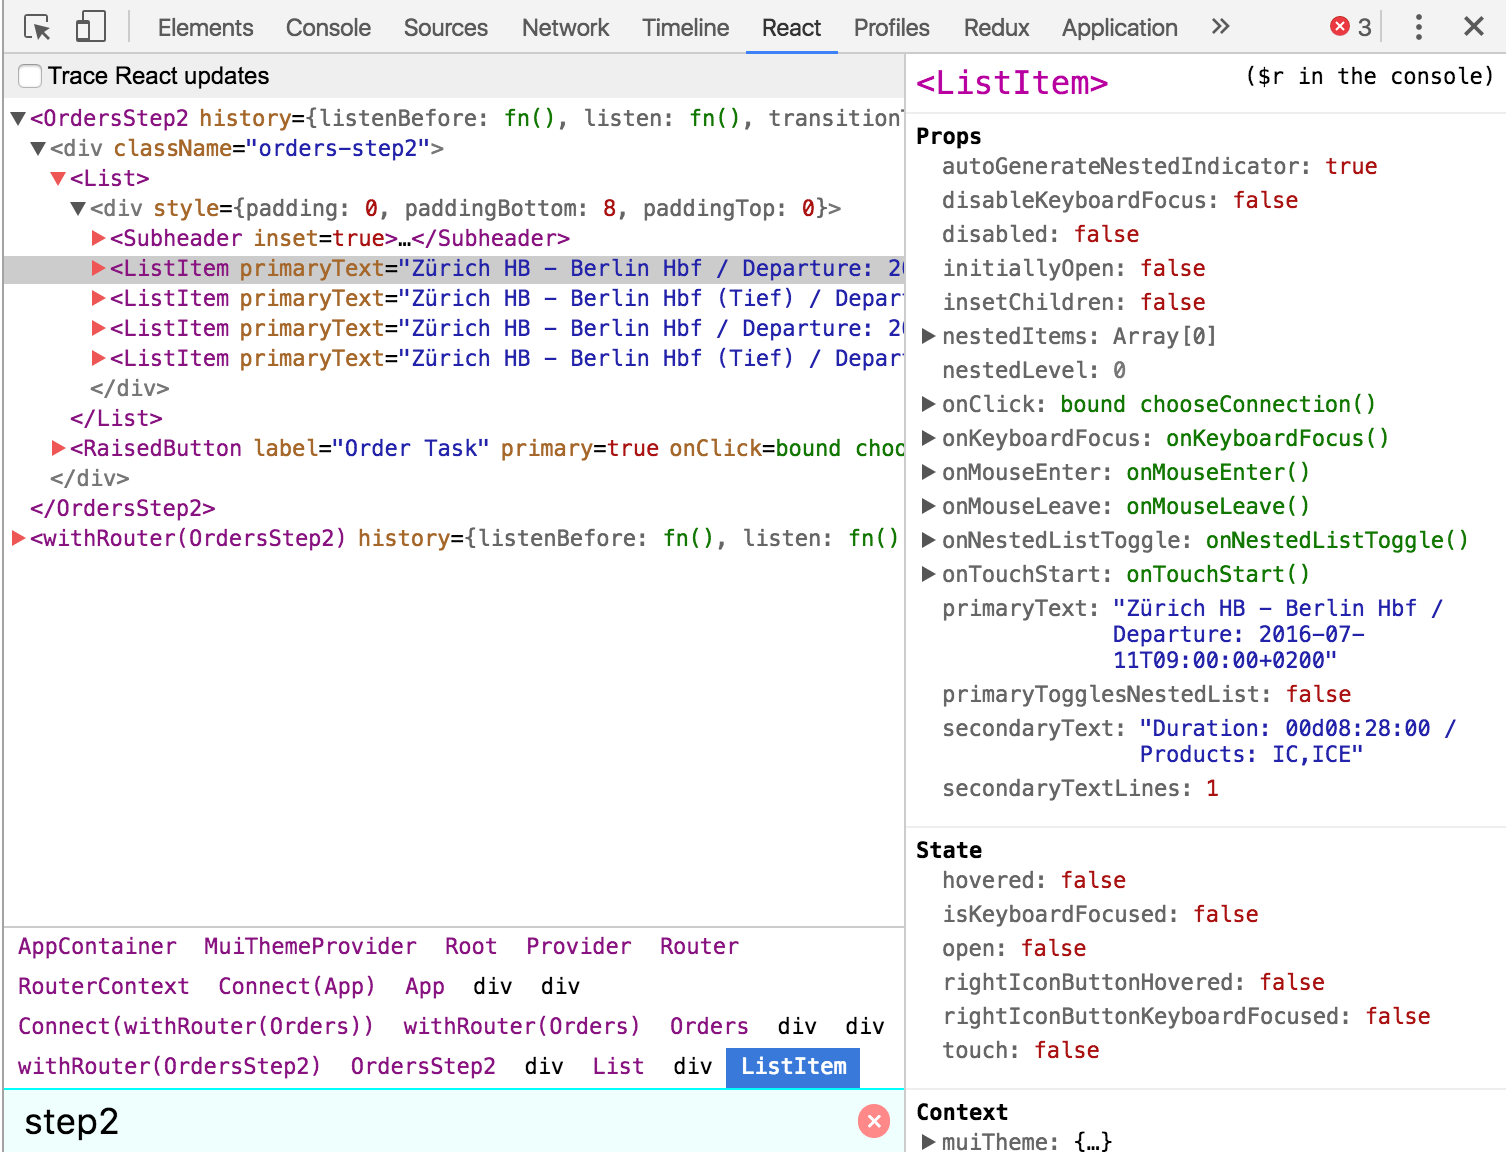
\includegraphics[width=0.88\textwidth]{images/reactext.png}
	\caption{React Browser Erweiterung}
	\label{fig:reactext}
\end{figure}

\subsubsection{Redux Erweiterung}
Die Redux Browser Erweiterung zeichnet alle ausgeführten Aktionen auf und listet diese auf einer Zeitachse auf. Die Aktionen können inspiziert und wieder rückgängig gemacht werden. Es wird aufgezeigt, wie der Zustand des \textit{Stores} vor und nach der Aktion aussieht. In Abbildung \ref{fig:reduxext} ist die Ansicht der Redux Browser Erweiterung zu sehen.

\begin{figure}[H]
	\centering
  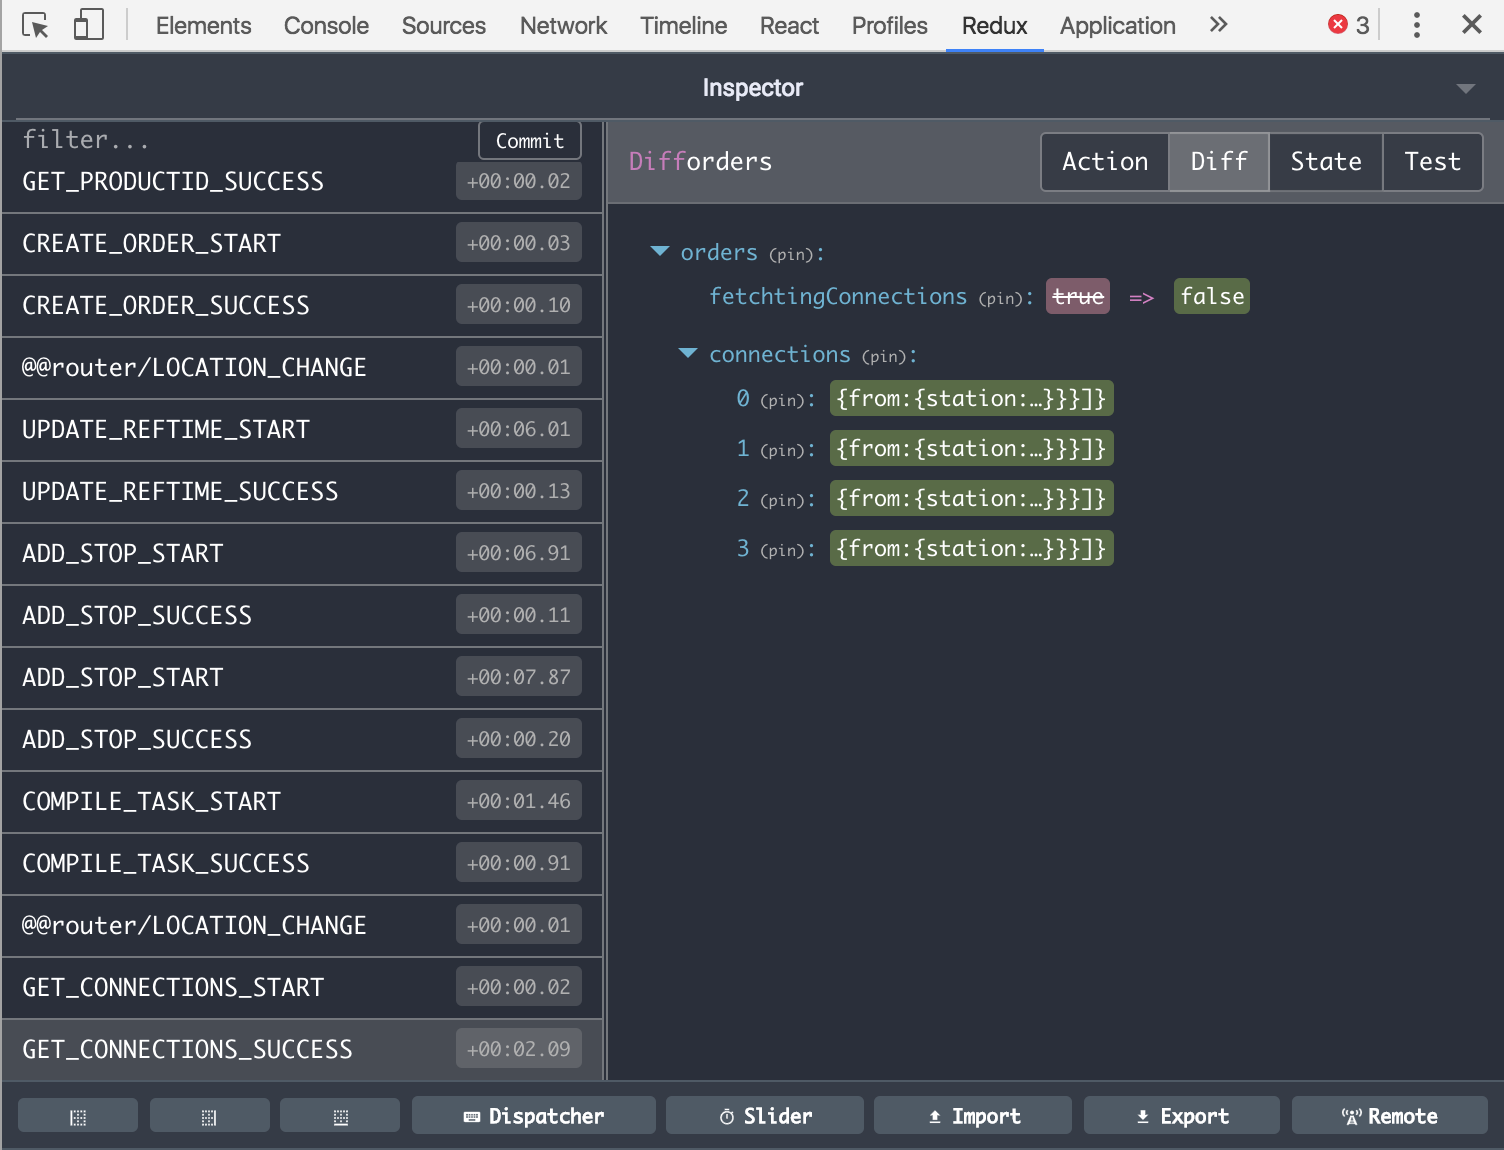
\includegraphics[width=0.88\textwidth]{images/reduxext.png}
	\caption{Redux Browser Erweiterung}
	\label{fig:reduxext}
\end{figure}


\subsection{Test Server}
Als Test Server wurde ein virtueller Ubuntu 16.04 Server verwendet. Als Webserver wurde nginx\footnote{\url{https://nginx.org}} verwendet. Der Webserver funktioniert als Proxy für den lokal laufende Node.js Webserver. Für Node.js wurde \textit{pm2}\footnote{\url{https://github.com/Unitech/pm2}} verwendet. Mit \textit{pm2} werden Node.js Prozesse überwacht, deren Standard Ausgabe abgefangen und gespeichert und im Falle eines Absturzes neu gestartet wird.

\section{Codebasis}
Für die Entwicklung wurde auf einer \textit{ToDo} Single-Page Applikation aufgebaut. Viele Software Frameworks oder Software Paradigmen werden in einem ToDo Projekt vorgestellt und lassen sich als Start für eigene Projekte verwenden. Im Rahmen dieser Bachelorarbeit wurde auf das \textit{ToDo-React-Redux} Projekt von Richard Park auf Github\footnote{\url{https://github.com/r-park/todo-react-redux}} zurückgegriffen. Das Projekt implementiert eine einfach ToDo Applikation mit React und Redux. Die Daten werden mit Firebase\footnote{Firebase ist ein \textit{Backend as a Service} Anbieter. \url{https://firebase.google.com/}} synchronisiert und benötigen deshalb eine asynchrone Handhabung. Dies ist hilfreich, weil die Kommunikation mit dem Mini-Backend auch asynchron stattfindet. Für das Mini-Backend ist bereits eine einfache express.js Applikationen vorhanden. Zusätzlich verwendet das Projekt Wekzeuge wie Webpack, Babel, React-Redux und ESLint, welche im Folgenden genauer beschrieben werden.

\subsection{Webpack}
Webpack\footnote{\url{https://github.com/webpack/webpack}} ist ein modernes Werkzeug, welches hilft eine grosse Codebasis in statische Dateien zu transformieren. Diese statischen Daten können dann zur Verwendung in einer produktiven Umgebung verwendet werden. Die neuste Version von JavaScript erlaubt es, Inhalte zu exportieren beziehungsweise zu importieren. Dadurch kann die Applikation in viele verschiedene Teile aufgeteilt werden, die am Anfang ihres Codeteils auf diejenigen Codeteile verweisen, die zusätzlich benötigt werden. Diese Abhängigkeiten werden von Webpack für einen erfolgreichen produktiven Einsatz gelöst. Zusätzlich ermöglicht Webpack mit sehr wenigen Zeilen einen lokalen Webserver zu starten. Im Folgenden ist die Konfiguration für den verwendeten lokalen Webserver.
\begin{lstlisting}[caption=Lokaler Webserver]
  config.devServer = {
    contentBase: './src',
    historyApiFallback: true,
    host: HOST,
    hot: true,
    port: PORT,
    publicPath: config.output.publicPath,
    stats: {
      cached: true,
      cachedAssets: true,
      chunks: true,
      chunkModules: false,
      colors: true,
      hash: false,
      reasons: true,
      timings: true,
      version: false
    },
    proxy: {
      '/api/v1/*': {
        target: 'http://localhost:3001',
        secure: false
      }
    }
  };
\end{lstlisting}
Dieser lokale Webserver ist nur für die SPA zuständig und reagiert nur auf deren Dateiänderungen während der Entwicklung. Für das Mini-Backend wird ein eigener lokaler Webserver verwendet, welcher nur auf Dateiänderungen im Mini-Backend reagiert. In einer produktiven Umgebung werden SPA sowie Mini-Backend vom gleichen Webserver bedient, was zum Problem führt, dass während der Entwicklung die Anfragen an das Mini-Backend umgeleitet werden müssen. In Webpack ist dies mit dem Parameter Proxy möglich, welcher alle Anfragen auf eine gewisse URL umleitet.


\subsection{Babel}
Babel\footnote{\url{https://babeljs.io/}} ist ein JavaScript transpiler, der es erlaubt, die neuste Version von JavaScript für alle Browser ausführbar zu machen. Obwohl die neuste Version von JavaScript bereits im Juni 2015 veröffentlicht wurde, sind noch nicht alle Browserhersteller in der Lage all diese Erneuerungen in ihren Browser auszuführen. Babel transpiliert diesen neuen Code in bekannten JavaScript ES5 Code, der selbst von älteren Browsern ausgeführt werden kann. Babel wird mit Webpack verwendet und hat den grossen Vorteil, dass die Codebasis auf viele neue und bessere Programmiereigenschaften zugreifen kann.

\subsection{React-Redux}
React-Redux\footnote{\url{https://github.com/reactjs/react-redux}} ist eine Erweiterung für React und Redux, welche die beiden Frameworks miteinander verbindet. Redux sieht vor dass es nur einen \textit{Store} gibt, der alle Daten für die gesamte Applikation beinhaltet. Dieser Store wird auf der obersten Ebene von React definiert und einer Provider Komponente übergeben.

\begin{lstlisting}[caption=Root Komponente]
export default function Root({history, onEnter, store}) {
  return (
    <Provider store={store}>
      <Router history={history}>
        <Route component={App} onEnter={onEnter} path="/">
          <IndexRoute component={Home} />
          <Route component={Orders} path={ORDERS_PATH}>
            <IndexRoute component={OrdersStep1} />
            <Route component={OrdersStep2} path={ORDERS_PATH + '/step2'} />
            <Route component={OrdersStep3} path={ORDERS_PATH + '/step3'} />
            <Route component={OrdersStep4} path={ORDERS_PATH + '/step4'} />
          </Route>
          <Route component={SignIn} path={SIGN_IN_PATH} />
          <Route component={Tasks} path={TASKS_PATH} />
        </Route>
      </Router>
    </Provider>
  );
}
\end{lstlisting}

Damit dieser \textit{Store} nicht durch alle Subkomponenten durchgereicht werden muss, wird mit react-redux das Werkzeug \textit{connect} zur Verfügung gestellt. Damit ist es möglich, bei der Definition einer Komponente zu definieren, welcher Teil des \textit{Stores} in der Komponente bereit gestellt werden soll. Im Folgenden Codebeispiel ist zu sehen, wie ein Teil des \textit{Stores} der Orders Komponente mit \textit{connect} zur Verfügung gestellt wird.
\begin{lstlisting}[caption=connect im Einsatz]
export default connect(state => {
  return {
    orders: state.orders
  };
}, Object.assign({}, ordersActions))(Orders);
\end{lstlisting}

\subsection{ESLint}
ESLint\footnote{\url{http://eslint.org/}} ist ein JavaScript linter, der auf Plugins aufbaut. Im Gegensatz zu anderen Codelintern ist ESLint in der Lage, JSX Code zu interpretieren und eignet sich deshalb für React Softwareprojekte. Ein Linter trägt stark zur Qualität und Verwaltbarkeit von Softwareprojekten bei.

\section{Entwicklungsprozess}
\subsection{Mini-Backend}
Das express.js wurde um eine isolierte Schnittstelle erweitert, die unter der URL (/api/v1/*) die definierten Methoden des Mini-Backends zur Verfügung stellt. Methoden, die nur Daten zurückliefern sind mit HTTP GET aufzurufen, alle anderen Methoden müssen mit HTTP POST aufgerufen werden. Jede Schnittstellen-Methode, die eine Anfrage an LoBo sendet, benötigt eine gewisse Bearbeitung, welche im Folgenden beschrieben ist.

\subsubsection{LoBo Anfragen}
Für eine erfolgreiche Anfrage an LoBo müssen gewisse Eigenschaften erfüllt sein. Die Parameter müssen als Strings gesendet werden. Zusätzlich zur gewünschten Anfrage und den benötigten Parametern muss das gewünschte Antwortsformat mitgeschickt werden. Die Parameter müssen in einem URL-Enkodierten Form gesendet werden. Im Header der Anfrage werden die Client Id und den Hash der zu sendenden Parameter erwartet. Für all dies Anforderungen wurde eine Methode geschrieben, welche diese Aufgaben übernahm.

\begin{lstlisting}[caption=Methode für LoBo Anfragen]
function createLoboRequest(action, params = {}) {

  // Ensure that all parameters are strings
  for (let key in params) {
    if ({}.hasOwnProperty.call(params, key)) {
        params[key] = String(params[key]);
    }
  }

  // Combine Parameters with defaults
  const postArray = Object.assign({
    action: action,
    clientIp: '127.0.0.1',
    responseFormat: 'json'
  }, params);

  // Create Hash
  const shaObj = new JsSHA('SHA-256', 'TEXT');
  shaObj.setHMACKey(CONFIG.LOBO_API_PRIVATE_KEY, 'TEXT');
  shaObj.update(JSON.stringify(postArray));

  return {
    url: CONFIG.LOBO_API_URL,
    method: 'POST',
    headers: {
      'X-Client-Id': CONFIG.LOBO_API_CLIENT_ID,
      'X-Public-Hash': shaObj.getHMAC('HEX')
    },
    form: postArray
  };
}
\end{lstlisting}

\subsubsection{Request Promises}
Gewisse Methoden wie die in Kapitel \ref{sec:architektur} beschriebene \textit{verifyaddress}, benötigen viele Anfragen an LoBo und andere Schnittstellen. Für die Handhabung dieser Abfolge von verschieden Anfragen wurde ein Node.js Modul\footnote{NPM Module request-promise \url{https://github.com/request/request-promise}} verwendet, welches erlaubt Anfragen als \textit{Promise} auszuführen. JavaScript \textit{Promise} sind Funktionen, die positiv oder negative aufgelöst werden können. Zusätzlich sind sie in der Lage in Serie zu funktionieren. Dies erlaubt, dass auf eine asynchrone Antwort gewartet und dann erst die nächste Aktion ausgeführt wird. Gleichzeitig bleibt der Code sehr übersichtlich und ein Fehler kann jederzeit abgefangen werden.


\subsubsection{Polygone}
Die Polygone werden benötigt um herauszufinden, ob und welche Bahnhöfe hinzugefügt werden sollen. Mit LoBo lässt sich zwar eine Adresse verifizieren, aber es gibt keine Möglichkeit herauszufinden, ob zwei Adressen im selbem Versorgungsgebiet liegen. Obwohl LoBo in der Lage wäre, die vorhandenen definierten Versorgungsgebiete auszugeben, hatte die Version von LoBo, welche im Rahmen dieser Bachelorarbeit verwendet wurde, diese Funktion deaktiviert. Für den Prototypen wurde für die zwei Städte Zürich und Berlin eigene Polygone erstellt. Mit der Web Applikation iso4app\footnote{\url{http://iso4app.net/}} können Erreichbarkeitskarten erstellt werden. Mit einer Zeitangabe und einem Startort wird ein Polygon erstellt, welches für die Punkte die Längen und Breitengrade abspeichert. Für Zürich und Berlin wurden die Polygone mit einem Zeitradius von 60 Minuten erstellt. Die einzugebenden Adressen wurden mit Hilfe von Google Maps automatisch vervollständigt. Dies hatte den Vorteil, dass der Längen- und Breitengrad der Adresse ebenfalls bekannt war. Im Mini-Backend wurden zwei Node.js Module\footnote{Polygon.js \url{https://github.com/tmpvar/polygon.js}, Vec2.js \url{https://github.com/tmpvar/vec2.js}} hinzugefügt, welche halfen herauszufinden, ob sich ein Punkt in einem Polygon befand oder nicht.


\subsection{SPA}
\subsubsection{Aktionen}
Aktionen, welche in Redux definiert sind, werden synchron ausgeführt. Um eine asynchrone Anfrage mit Redux an das Mini-Backend auszuführen, müssen mehrere Aktionen definiert werden. Bevor die Anfrage ausgeführt wird, wird dem \textit{Dispatcher} eine START Aktion übergeben. Sobald die Antwort vom Mini-Backend zurückkommt, wird je nach Status der Antwort die SUCCCES Aktion für eine erfolgreiche Anfrage oder die ERROR Aktion für eine fehlgeschlagene dem \textit{Dispatcher} übergeben. Im \textit{Reducer} wird beim Empfang der START Aktion ein Flag gesetzt, welches aussagt, dass eine asynchrone Aktion ausgeführt wird. Beim Empfang der erfolgreichen beziehungsweise fehlgeschlagenen Aktion wird dieses Flag wieder zurück gesetzt. Im Folgenden ist dieses Redux Verhalten an der Aktion, welche die verfügbaren Bahnverbindungen lädt, dargestellt.

\begin{lstlisting}[caption=Aktion getConnections]
export function getConnections(from,to,date,pickup) {
  return dispatch => {
    dispatch({type: GET_CONNECTIONS_START, payload: null});
    const connections = {
      'method': 'POST',
      'headers': {'Content-Type': 'application/json'},
      'body': JSON.stringify({from, to, date, pickup})
    };
    return fetch('/api/v1/connections',connections)
      .then(data => data.json())
      .then(json => {
        dispatch({
          type: GET_CONNECTIONS_SUCCESS,
          payload: json
        });
      })
      .catch(error => {
        dispatch({
          type: GET_CONNECTIONS_ERROR,
          payload: error
        });
      });
  }
}
\end{lstlisting}

Die Methode \textit{getConnections} wird mit den Argumenten from, to, date und pickup aus einer Komponente aufgerufen. Zuerst wird der Aktionstyp \textit{GET\_CONNECTIONS\_START} auf Zeile drei an den \textit{Dispatcher} übergeben. Auf Zeile vier bis acht wird die HTTP POST Anfrage zusammen gestellt. Auf Zeile neun wird mit \textit{fetch} die Anfrage ausgeführt und sobald eine Antwort zurückkommt auf Zeile zehn von JSON in ein JavaScript Objekt umgewandelt. Dieses wird mit dem Aktionstyp \textit{GET\_CONNECTIONS\_SUCCESS} auf Zeile 12 bis 15 dem \textit{Dispatcher} übergeben. Sollte ein Fehler zurückkommen, passiert das gleiche mit dem Aktionstyp \textit{GET\_CONNECTIONS\_ERROR} auf Zeile 18 - 21.

\begin{lstlisting}[caption=Reducer getConnections]
    case GET_CONNECTIONS_START:
      return Object.assign({}, state, {fetchingConnections: true});
    case GET_CONNECTIONS_SUCCESS:
      return Object.assign({}, state, {
        fetchingConnections: false,
        connections: action.payload
      });
    case GET_CONNECTIONS_ERROR:
      return Object.assign({}, state, {
        fetchingConnections: false,
        connections: []
      });
\end{lstlisting}

Sobald der \textit{Reducer} den Aktionstyp \textit{GET\_CONNECTIONS\_START} erkennt, wird das Attribut fetchingConnection auf Wahr geschaltet. Wenn eine positive Antwort zurückkommt, wird der Aktionstyp \textit{GET\_CONNECTIONS\_SUCCESS} empfangen und die Bahnverbindungen im \textit{Store} unter \textit{connections} abgespeichert. Sollte eine negative Antwort zurückkommen wird \textit{connections} mit einem leeren Array überschrieben.

\subsubsection{Komponenten}
Komponenten bestehen aus einer JavaScript Klasse, welche von den React Komponenten erben. Die einzige Methode, welche zwingend ist, ist die \textit{render} Methode. Die \textit{render} Methode wird beim Laden der Single-Page Applikation ausgeführt und das zurückgegebene JSX im Browser dargestellt.

\begin{lstlisting}[caption=Render Methode der OrderStep2 Komponente]
  renderConnections() {
    const { orders } = this.props;
    if(orders.connections.length > 0) {
      return (
        <List>
          <Subheader inset={true}>Connections</Subheader>
          {orders.connections.map(connection => {
            return (
              <ListItem
                primaryText={connection.from.station.name + ' - ' + connection.to.station.name + ' / Departure: ' + connection.from.departure}
                secondaryText={'Duration: ' + connection.duration + ' / Products: ' + connection.products.join()}
                onClick={this.chooseConnection.bind(this,connection)}
              />
            );
          })}
        </List>
      )
    }
  }

  render() {
    return (
      <div className="orders-step2">
        {this.renderConnections()}
        <RaisedButton label="Order Task" primary={true} onClick={this.chooseConnection.bind(this)} />
      </div>
    );
  }
\end{lstlisting}

In der \textit{render} Methode können andere Methoden aufgerufen werden, welche wiederum JSX zurück geben. In der \textit{renderConenctions} Methode wird über ein Array aus dem \textit{Store} iteriert, welches für jede Bahnverbindung ein \textit{ListItem} mit den entsprechenden Eigenschaften zurück gibt.

